%!TEX root = ../dissertation.tex
\begin{savequote}[75mm]
The relationship between theorists and experimentalists is like that between a truffle farmer and his pig%If it's stupid but it works, it isn't stupid.
\qauthor{Howard Georgi}
\end{savequote}

\chapter{The Standard Model Higgs and Colider Event Variables}
\label{ch:theory}

\newthought{Much has been said} about the so-called Standard Model (SM) of particle physics, so we will try to keep this discussion as brief and (hopefully) as error free as possible.% before moving onto a discussion of the treatment of kinematic variables in collider events, including the two novel schemes considered in this thesis, the Lorentz Invariants (LI) and RestFrames (RF) variables.
  The discussion of Higgs physics follows the notation of \cite{pdg} Chapter 11.

\section{The Standard Model Higgs Boson}
The generic scalar Lagrangian potential (the kinetic term will be addressed later) for a scalar in the SM is:
\begin{equation}
V\left(\Phi\right) = m^2\Phi^\dagger\Phi+\lambda\left(\Phi^\dagger\Phi\right)^2
\end{equation}
where $\Phi$ is the Higgs field, a complex scalar doublet under $SU\left(2\right)$.  Its four degrees of freedom are typically decomposed as follows:
\begin{equation}
\Phi = \frac{1}{\sqrt{2}}} \left(\begin{array}{c} \sqrt{2}\phi^+\\ \phi^0 + ia^0 \end{array}\right)
\end{equation}
$\phi^+$ is the complex charged component of the Higgs doublet, and $\phi^0$ and $a^0$ are the CP-even and CP-odd neutral components, resepectively.

If the sign of $m^2\Phi^\dagger\Phi$ is negative, $\Phi$ acquires a \emph{vacuum expectation value} or VEV:
\begin{equation}
\left<\Phi\right> = \frac{1}{\sqrt{2}}} \left(\begin{array}{c} 0 \\ \sqrt{\frac{2m^2}{\lambda}} \end{array}\right)
\end{equation}
with this value typically denoted $v=\sqrt{2m^2/\lambda}=\sqrt{\sqrt{2}G_F}\approxsim246$ \GeV\,(with the coupling of the 4-Fermi effective theory of weak interactions measured through experiments involving muon decay), and $\phi^0$ is rewritten as $\phi^0=H+v$.

It is this non-zero VEV that induces spontaneous symmetry breaking in the SM's gauge (local) symmetry group of $SU\left(3\right)_C\times SU\left(2\right)_L\times U\left(1\right)_Y$ since the VEV does not respect the $SU\left(2\right)_L\times U\left(1\right)_Y$ symmetry of the Lagrangian (i.e. $\left<\Phi\right>$ is not invariant under a gauge transformation of this group).  Three of the four generators of this subgroup are spontaneously broken, which implies the existence of three massless Goldstone bosons, which are in turn ``eaten'' by linear combinations of the $W^a$ and $B$ bosons to form the longitudinal components of the familiar $W^{\pm}$ and $Z$ bosons, with the last generator giving rise to the usual, unbroken $U\left(1\right)_{EM}$ symmetry and its massless photon, $A$, as well as the scalar Higgs boson $H$.  To see this one starts with the full Higgs SM Lagrangian (kinetic minus potential only)
\begin{equation}
\mathcal{L}_{Higgs}=\left(D_{\mu}\Phi\right)^\dagger\left(D_{\mu}\Phi\right)-V\left(\Phi\right),\; \D_{\mu}\Phi = \left(\partial_{\mu}+ig\sigma^a W^a_\mu + ig'YB_\mu/2\right)\Phi
\end{equation}
One simply plugs in the reparametrized $\Phi$ with $\phi^0=H+v$, collects the terms involving $v$ together with the appropriate $W$ and $B$ kinetic terms to extract:
\begin{equation}
M_W^2=\frac{g^2v^2}{4},\;M_Z^2=\frac{\left(g'^2+g^2\right)v^2}{4}
\end{equation}
This is left as an exercise for the reader; this exercise also makes it manifest that the Higgs couplings with the $W^\pm$ and $Z$ scale quadratically with their masses.  Since the Higgs field also respects the $SU\left(3)_C$ color symmetry, the eight gluons are also left massless, and the $H$ is left interacting with photons and gluons primarily through heavy quark loops.

\begin{figure}[!htbp]\captionsetup{justification=centering}
  \centering
  \includegraphics[width=0.75\linewidth]{figures/sm_particles}
  \caption{The fundamental particles of the Standard Model.  IC: \cite{smcartoon}}
  \label{fig:smparticles}
\end{figure}
The Higgs is often introduced to the public at large as the mechanism through which fundamental fermions (enumerated in Figure \ref{fig:smparticles}) acquire mass---this is through the Yukawa interactions of the Higgs:
\begin{equation}
\mathcal{L}_{Yukawa}=-\hat{h}_{d_{ij}}\bar{q}_{L_i}\Phi d_{R_j}} - \hat{h}_{u_{ij}}\bar{q}_{L_i}\tilde{\Phi} u_{R_j}} -\hat{h}_{l_{ij}}\bar{l}_{L_i}\Phi e_{R_j}} + h.c.
\end{equation}
where $\tilde{\Phi}=i\sigma_2\Phi^*$, $q_L$ ($l_L$) and $u_R$, $d_R$ ($e_R$) are the quark (lepton) left-handed doublets and right handed singlets of the weak $SU\left(2\right)_L$ group, with each term parametrized by a $3\times3$ matrix in family space (also known as the fermion generations).  The neutrinos have been purposely omitted since the mechanism that generates their mass is as of yet unknown, though these Yukawa interactions could have a non-zero contribution.  Once the Higgs VEV value is known and the Yukawa interaction matrices $\hat{h}_{f_{ij}}$ ($i,j\in\left{1,2,3\right}$) are diagonalized, the fermion masses can simply be written as $m_{f_i}=h_{f_i}v/\sqrt{2}$.  The SM has no motivation for any of these masses.

Note that from $\mathcal{L}_{Yukawa}$, it is easy to see that the Higgs couplings with fermions scale linearly with fermion mass.  Higgs self-couplings and beyond the standard model (BSM) Higgs scenarios are beyond the scope of this thesis.

\section{Higgs Boson Production and Decay at the Large Hadron Collider}
The leading order Feynmann diagrams for the four dominant modes of Higgs production at the LHC are shown in Figure \ref{fig:hprod}, each described briefly in turn.
\begin{figure}[!htbp]\captionsetup{justification=centering}
  \centering
  \includegraphics[width=0.65\linewidth]{figures/higgs_proudction}
  \caption{Dominant Higgs production modes.}
  \label{fig:hprod}
\end{figure}
The dominant process, accounting for some 87\% of Higgs production at the nominal LHC center of mass energy of 14 \tev, is gluon-gluon fusion (ggF), shown in Figure \ref{fig:hprod} (a).  At high center of mass energies, most of a proton's momentum is predominantly carried by sea gluons (as opposed to the constituent valence quarks associated with the hadron's identity).  This, along with the difficulties associated with high luminosity antiproton beam production, is why the LHC was designed as a proton-proton collider instead of a proton-antiproton collider (like the Tevatron).  As mentioned above, the Higgs does not couple directly to gluons but must instead be produced through the fermion loop shown in the figure.  The heaviest fundamental fermion by far is the top quark, with $m_t=173$ \gev, so top loops dominate this process.  While not particularly relevant for this thesis, about 14\% of events in the 2-lepton channel of the $H\to b\bar{b}$ analysis are ggF initiated.

The next most prevalent process is vector boson fusion (VBF), where vector bosons ($W$ or $Z$, denoted generically as $V$) from quarks in the colliding quarks ``fuse'' to form a Higgs.  These quarks typically form jets in the forward region, which provides a unique signature for this process.  This process is not relevant for this thesis.

The third leading process is ``Higgsstrahlung'' or Higgs production in association with a vector boson, often simply $VH$ production.  In this process, a quark-antiquark pair in the colliding protons forms an energetic vector boson, which then radiates a Higgs (this is similar to photon emission of accelerating electrons, called ``bremsstrahlung,'' hence the name).  Some fraction of the time (about 21\% of the time for $WH$ and 6.7\% of the time for $ZH$), the energetic $V$ will decay leptonically (i.e. into a decay involving an electron or a muon), which provides a unique and triggerable signature for this process.  Another 20\% of the time for $ZH$ production, the $Z$ will decay to neutrinos, which are not absorbed by detectors and show up as missing transverse energy (\met), another triggerable singature.  This ability to trigger and require that this leptonic signature be consistent with a $V$ allows one to significantly reduce the impact of multijet background (a very common generic processes at the LHC) on analysis.  Hence, this is the process of primary importance to this thesis.

The final important Higgs production process is $t\bar{t}H$ production, the box diagram in Figure \ref{fig:hprod} (d).  Again, the top pair provides a useful signature for analysis.  This, like VBF, is also not considered in this thesis.


\begin{figure}[!htbp]\captionsetup{justification=centering}
  \centering
  \includegraphics[width=0.55\linewidth]{figures/higgsbr}
  \caption{Higgs decay modes as a function of its mass; a line has been drawn at the observed Higgs mass of 125 \gev.}
  \label{fig:hbr}
\end{figure}

Once the Higgs has been produced, it can decay in a number of ways, as shown in Figure \ref{hbr}.  By far the most dominant decay mode of the Higgs is to $b\bar{b}$ at 58\% of all decays.  This $b$-quark pair then hadronizes into two $b$-jets (for a more thorough discussion of jets and $b$-jets in particular, see Section \ref{sec:jets}).  However, many processes at the LHC create pairs of $b$-jets with invariant masses consistent with the Higgs have much higher production rates (\tt\,production at the LHC is in the neighborhood of hundreds of pb), so a clear process signature is necessary to study $H\to b\bar{b}$ production at the LHC.  This is why the bulk of search efforts have focused on $VH$ production.  A summary of Higgs production cross sections and simple extrapolations to raw numbers of Higgs bosons produced for $VH$ for leptonically decaying $V$ is shown in Table \ref{tab:xsec}

\begin{table}[!htbp]
\begin{center}
\begin{tabular}{lccccc}
\hline\hline
\sqrt{s} (\TeV) & ZH & WH & ggF & total \sigma & $N_{V_{\to\ell|\nu} H}$ \\
\hline
 7 & $0.34^{+4\%}_{-4\%}$ & $0.58^{+3\%}_{-3\%}$ & $15.3^{+10\%}_{-10\%}$ & 17.5 & 4.7 \fb\to 589\\
 8 & $0.42^{+5\%}_{-5\%}$ & $0.70^{+3\%}_{-3\%}$ & $19.5^{+10\%}_{-11\%}$ & 22.3 & 20.3 \fb\to 3 100\\
13 & $0.88^{+5\%}_{-5\%}$ & $1.37^{+2\%}_{-2\%}$ & $44.1^{+11\%}_{-11\%}$ & 50.6 & 36.1 \fb\to 11 100\\
14 & $0.99^{+5\%}_{-5\%}$ & $1.51^{+2\%}_{-2\%}$ & $49.7^{+11\%}_{-11\%}$ & 57.1 & 1000 \fb\to 343 000\\
\hline
\hline
\end{tabular}
\end{center}
\caption{Cross sections for processes important to the SMVHbb analysis and the total Higgs cross section as a function of center of mass energy.  Also given are the total number of Higgs bosons produced for given luminosities through both $WH$ and $ZH$ processes.}
\label{tab:xsec}
\end{table}

\section{Collider Events and Event Level Variables}
Collision data in experiments like ATLAS is structured using what is known as the \emph{event data model}.  In this model, one collision corresponds to one event.  The raw data, the various tracks, energy deposits, and hits in the detector, undergo reconstruction (described at length in Chapter \ref{ch:object}) both through automated experiment-wide standards and through analysis-specific level selections, corrections, and calibrations.  The result of this considerable effort is a collection of labeled 4-vectors, representing the final state objects.  This is shown in Figure \ref{fig:recon}.

\begin{figure}[!htbp]\captionsetup{justification=centering}
  \centering
  \begin{subfigure}[t]{0.420000\textwidth}\centering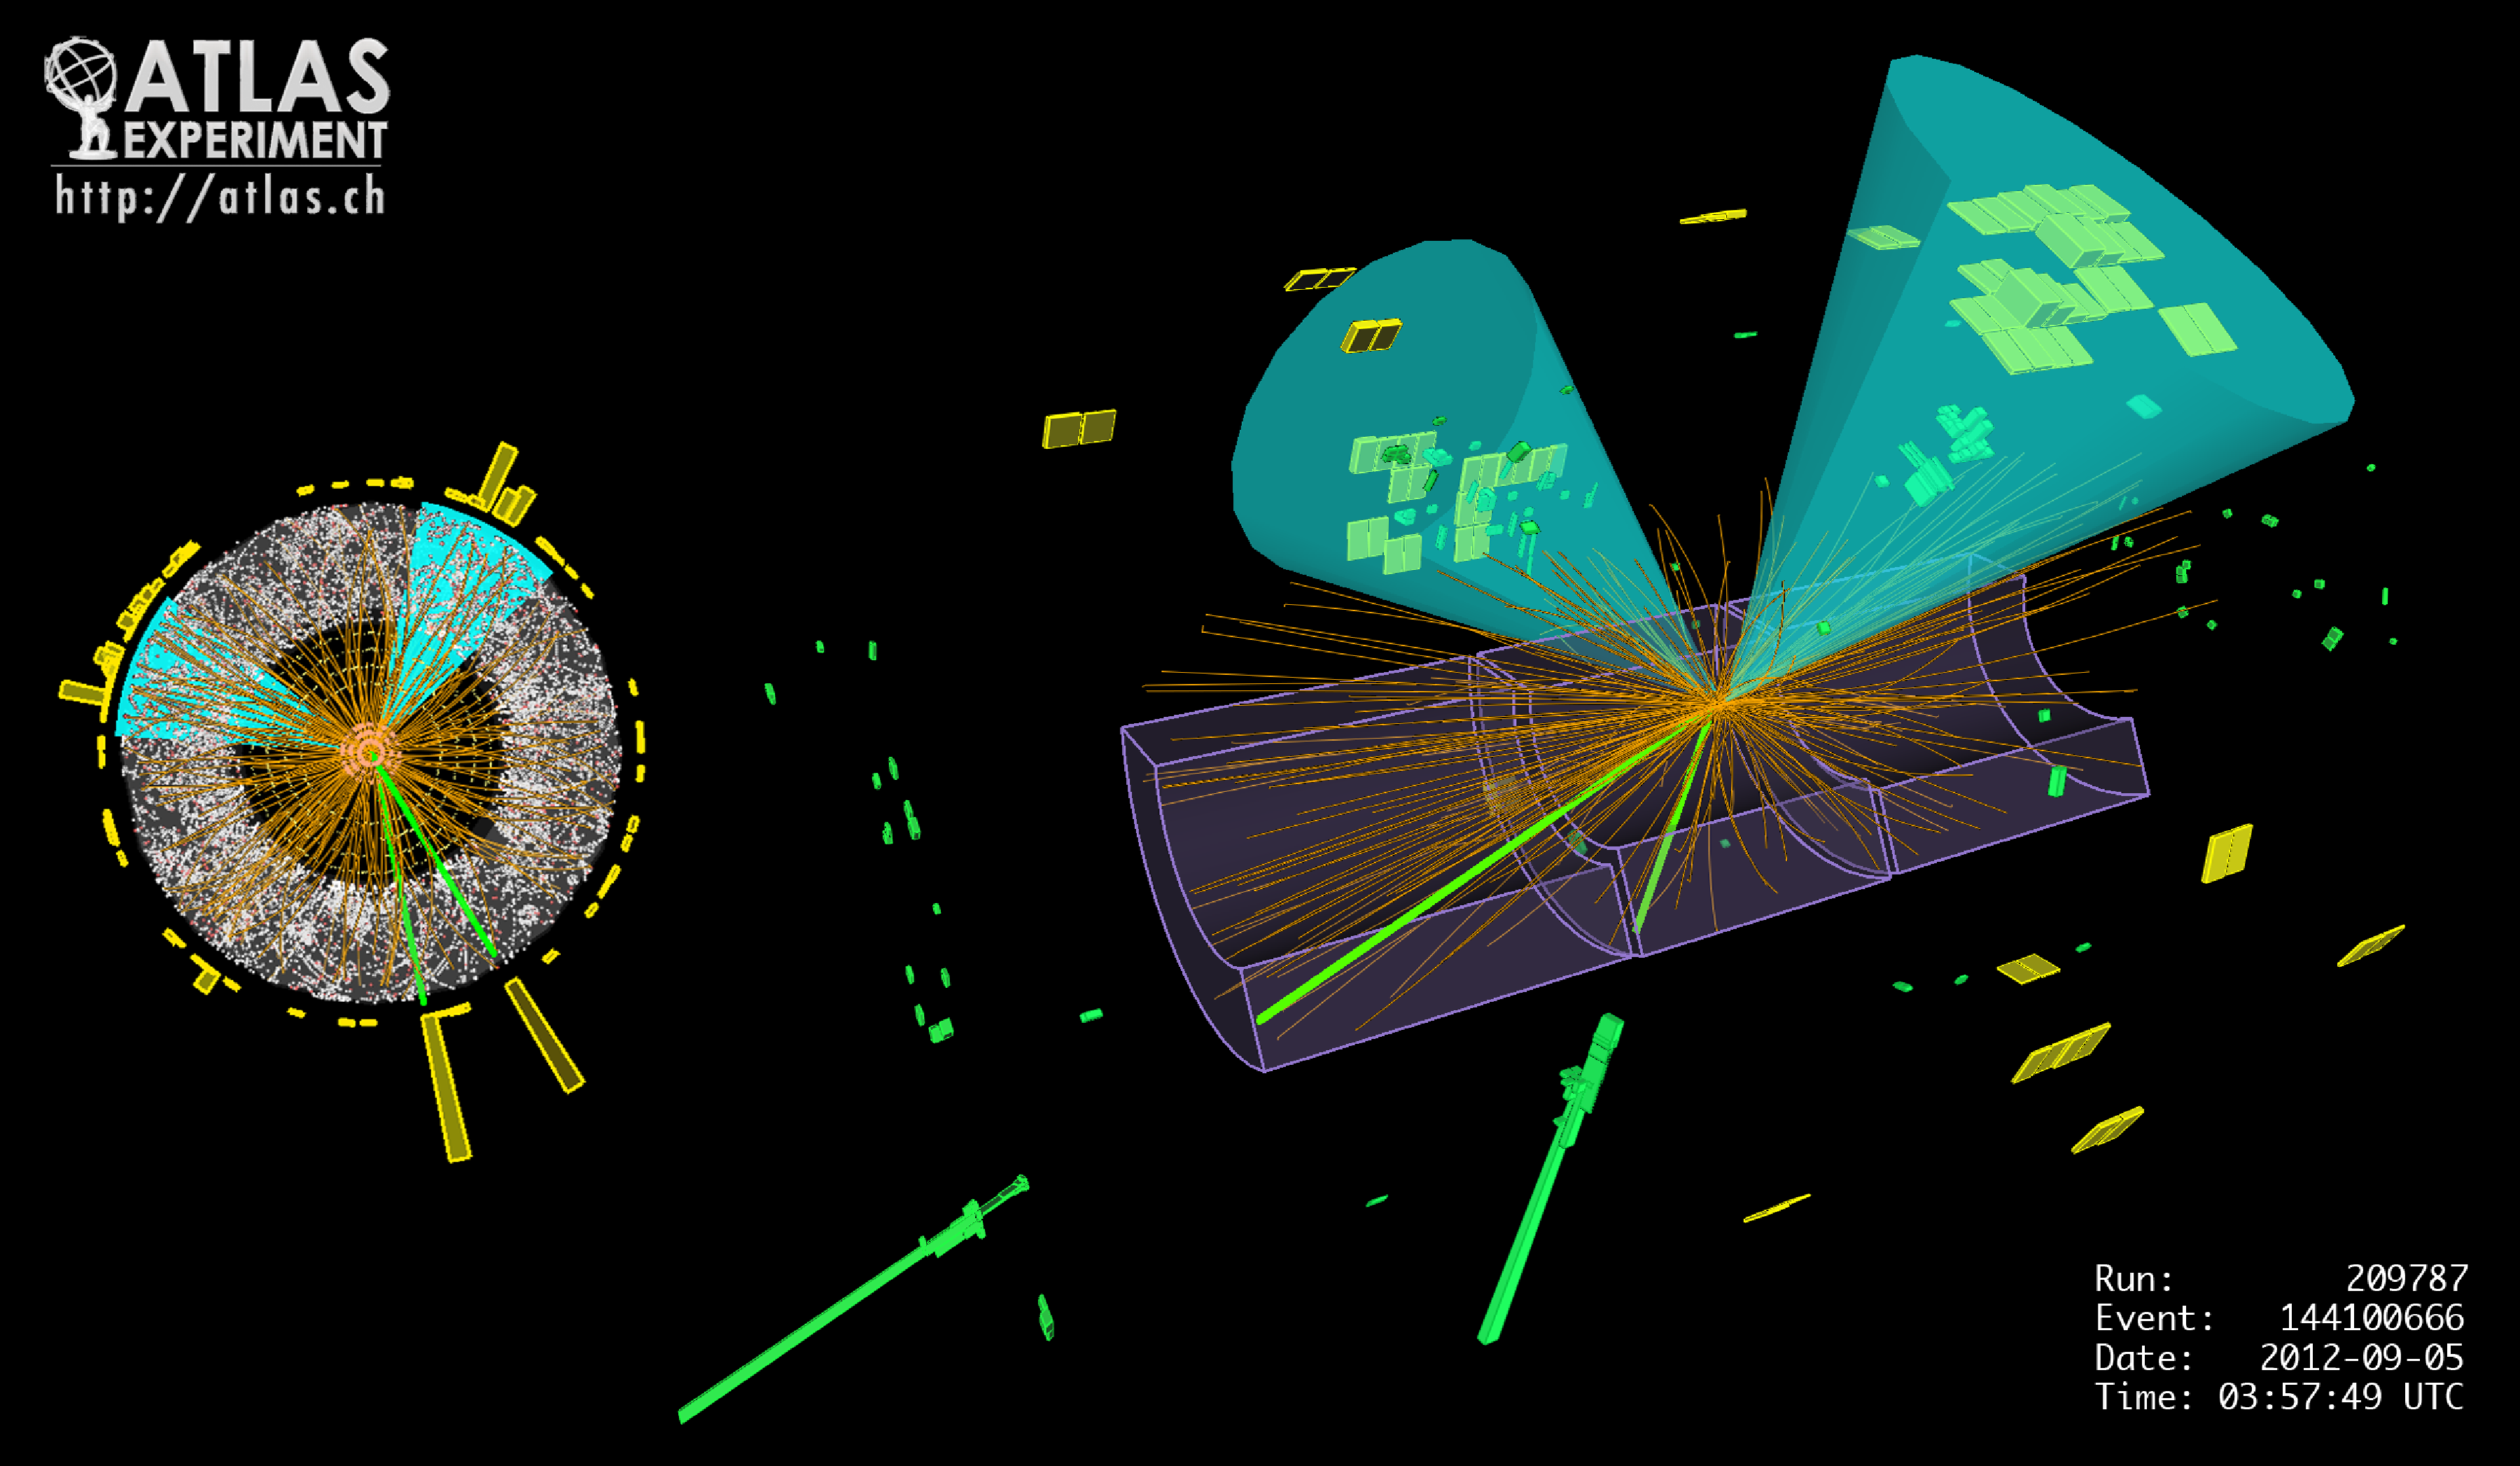
\includegraphics[width=\textwidth]{figures/atlas/atlas_3dzhllbb}}\caption{This}\end{subfigure}
  \begin{subfigure}[t]{0.420000\textwidth}\centering\includegraphics[width=\textwidth]{figures/zhllbb}}\caption{Stands in for this}\end{subfigure}
  \caption{Reconstruction in a nutshell}
  \label{fig:recon}
\end{figure}

In the process that is the focus of this thesis, every event utlimately is condensed into a lepton pair (two electrons or two muons), two or three jets\footnote{Sometimes more, though this is a small fraction of events, and the wisdom of this choice may be questioned}, all 4-vectors and a \met\, vector in the transverse plane.  Further selection then takes place to winnow down events into interesting regions of phase space hopefully more rich in signal-like events.  Once events are selected in a search like the one in this thesis, one then analyzes the data to test its consistency with some background only hypothesis to produce the usual significances quoted.  This can be done in various ways, with main approches being: a simple counting experiment (often referred to as the ``cut and count'' approach), a functional fit for excesses over a falling background spectrum (the so-called ``bump hunt'' used in analyses like the $H\to\gamma\gamm$ discovery channel), or the use of discriminant distributions as PDF's in a likelihood fit (the approach of this analysis).  These distributions can be simple counts (i.e. single bin distributions) in analysis regions, quantities of interest (the distribution of the invariant mass of the two $b$-jets in selected events with the greatest transverse momenta, $m_{bb}$, is used as a validation), or something more complicated like a multivariate analysis (MVA) discriminant.

\section{Characterization with Event-Level Variables}
This is where our story truly begins.  Traditionally, particle physicists have favored the approach of using distriubtions of physical variables since it is easier to develop ``physical intuition'' for what these distributions should ``look like'' during validation, so it is no surprise that as many LHC analyses have transitioned to using MVA techniques that these variables form the basis of many very robust physics results.  These variables do quite well summarize many of the main physics features of an event for the signal topology.  In \ZH\,events, for example, one wishes to characterize the $ZH$ system by using the lepton pair as a stand-in for the $Z$ and the $b$-jet pair as a stand-in for the $H$, and composite variables like \mbb\,and \mll\, can be used to check whether events are consistent with these objects.  There are also variables like \ptv\, that characterize the momentum scale of the event, angles like $\Delta R\left(b_1,b_2\right)$ and $\Delta\phi\left(V,H\right)$ that can be further used to characterize the overall ``shape'' of these events, and variables like \met\,that can discriminate against backgrounds like \tt\,that do not have a closed topology.

Nevertheless, the intuition based approach, with incremental addition of variables as they prove useful in the lifetime of an analysis's iterations, does beg the question of whether there is a more systematic way to treat this information.  There are clearly patterns to which variables are useful: these correspond to important information about the hypothesized physics objects and their relationships, so could there be some gain in finding a way to systematize the way these are found?  Such systematic, top-down approaches often promise to increase performance in two ways.  The first is by having higher descriptive power, often through some sophistocated treatment of the missing transverse energy in an event, \met.  \met\, is just a single number, and if there is just one invisible object in a desired event topology, using \met\,on its own often provides sufficient sensitivity.  In more complicated topologies with multiple invisible particles in the final state, for example in many supersymmetry searches, a more careful treatment of the missing energy is often necessary.

  The second means of improvement is through using a more orthogonal basis of description, which allows one to more efficiently use data and simulation samples.  A more orthogonal basis implies that variables contain less overlapping information with each other and so allow for a more efficient exploration of parameter space.  This means one can gain higher sensitivity from equivalent datasets using a more orthogonal basis.  To see why this might be the case, take an MVA discriminant for \ZH\,formed using only the classic variables $\Delta R\left(b_1,b_2\right)$ and \ptv.  In the \ZH\,topology, transverse mass of the $Z$ and $H$ (and hence the lepton pair and jet pair) are equivalent.  This means that at higher \ptv\, the $p_T$ of $b$-jets will also be higher, which in turn implies that they will have a smaller angle of separation and hence a smaller $\Delta R\left(b_1,b_2\right)$.  This correlation is not unity---each variable still does have information the other does not---but it is still very high.  Hence, when training an MVA, which in principle knows nothing about these variables other than some set limits, an undue number of training events will be wasted converging upon relations that could be known \emph{a priori}, and while this might be easy to hard code in for a two variable toy example, the dimensionality of any real discriminant makes this prohibitive.  An MVA that uses data (both actual and simulated) more efficiently will also tend to be more robust to variations, offering a potential avenue for reduction in the error on quantities of interest due to systematic uncertainties.  Details of how this plays out in a likelihood fit will are deferred to the discussion of the fit model used in the VHbb search in Chapter \ref{ch:fit}.

Many of these novel schemes are designed to explicitly address the first issue in channels where it is of paramount importance while having the second issue as something of a fringe benefit.  However, as the amount of data taken at the LHC grows, analyses will increasingly become systematics limited, so an exploration to the veracity of the second claim has great potential for the high luminosity era of the LHC.  The \ZH\,process offers a great setting for investigating this issue on its own since its closed topology largely mitigates any improvement from more sophistocated treatments of \met.  We introduce two of these more top-down approaches to event-level variables below: the ``Lorentz Invariant'' (LI) \cite{litalk} and ``RestFrames inspired'' (RF) \cite{rjr} varaiable schemes.  A broad overview of the concepts behind these schemes will be given here, with a more in-depth discussion of their implementation deferred until Chapter \ref{ch:mva}.


\section{Lorentz Invariants}
  The LI variables, first put forth by S. Hagebock and others \cite{litalk}, are based upon the fact that the four-vectors of an event are determined, all of the information in an event are encoded into their inner products (Lorentz invariant quantities, hence the name) and the angles between them.  This makes for 16 quantities in all: the ten inner products of the four vectors, the three Euler angles, and the three parameters specifying the boost of the $ZH$ system.  The masses of the four final state objects are not considered very useful and so can be removed to leave six meaningful inner products (the $_4C_2$ combinations between distinct final state four vectors).  Since these inner products can have an ill-defined physical interpretation and in order to help MVA training, each inner product is scaled by:
\begin{figure}[!htbp]\captionsetup{justification=centering}
  \centering
  \includegraphics[width=0.400000\linewidth]{figures/li2lep}
  \caption{Summary of LI variables in the \ZH\, topology.}
  \label{fig:rftree}
\end{figure}

\begin{equation}
\label{eqn:liip}
x\to\frac{x}{x+c}
\end{equation}
where $c$ is the mean of the distribution in the signal MC distribution.  These inner products are denoted \texttt{xi\_yj}, where \texttt{x} and \texttt{y} are either \texttt{j} (for jet) or \texttt{l} (for lepton) and the indices are either 0 (1) for the leading (subleading) object by $p_T$ in the event.

  The number of useful angles can be reduced by recognizing some symmetries inherent in the final state.  The symmetry around the beam axis eliminates one angle.  Furthermore, the boost of the $VH$ system is primarily in the beam direction ($z$) direction, marginalizing the utility of the transverse boost angles.  This leaves the boost in the $z$ direction, denoted \texttt{gamma\_ZHz}, and two angles chosen to be the angle between the $b\bar{b}$ system and the beam (\texttt{angle\_bb\_z}) and the angle between $\left(b_1+b_2\right)\times\hat{z}$ and $\left(b_1+b_2\right)\times\left(l_1+l_2\right)$ (\texttt{angle\_bbz\_bbll}).

These variables do contain a lot of information similar to the usual set: there are mass equivalents (\texttt{j0\_j1}$\leftrightarrow$\texttt{mBB}, and \texttt{l0\_l1}$\leftrightarrow$\texttt{mLL}) and angles.  Instead of individual final state object scales, there are the four jet/lepton inner products, though this correspondence (and indeed any physical intepretation) is far from clear.  An important advantage of the LI variable set is that all of the variables are in it are orthogonal in the signal case by construction.  A drawback of this framework in a completely closed final state is that there is no way to treat $E_T^{miss}$ in a Lorentz invariant way.  %In practice, however, it is found that the $E_T^{miss}$ has correlations comparable to other correlations between variables (cf. Figure \ref{fig:2jet-hiptv-correlations} (b) and (e)).
  There is also no prescription for any additional jets in the event beyond the two $b$-tagged jets.  They are simply ignored in these variable calculations since the fiducial analysis requirement of exactly two $b$-tagged jets elminates any combinatoric ambiguity.  

Perhaps a more troubling weakness of the Lorentz Invariants approach is that it is not generically applicable to all analysis channels.  The LI concept was initially formulated for sensitivity improvement in the 1-lepton channel.  In this case, the \met\, has a natural interpretation as the transverse momentum of the single neutrino in the signal topology.  Using the constraint of a massless neutrino, there is only one free parameter remaining, which is chosen to the be the neutrino's longitudinal momentum.  Following the discussion in \cite{litalk}, we first guess the neutrino energy in its rest frame and then boost to the lab frame:
\begin{equation}
\left<E_\nu\right>=\frac{1}{4}m_{WH}\implies \left<p_z^{\nu}\right>=\beta\gamma\left<E_\nu\right>=\frac{p_z^{WH}}{m_{WH}}\left<E_\nu\right>=\frac{1}{4}p_z^{WH}
\end{equation}
Finally, assuming energy and momentum in aggregate are equally shared among final state constitutents, we arrive at
\begin{equation}
\left<p_z^{\nu}\right>=\frac{1}{4}\times \frac{4}{3}\left(p_z^l+p_z^{j0}+p_z^{j1}\right)
\end{equation}
Nevertheless, there is no straightforward way to generalize this to the 0-lepton case, as there are twice as many degrees of freedom, making such a simple and intuitive guess impractical, or at least not immediately obvious.

This concept of rest frames and boost is actually the central tenant of the RestFrames variables, which can be used to construct variables for generic decay trees and to which we now turn.

\section{RestFrames Variables}
The RestFrames variables \cite{rjr}, calculated using the software package of the same name, is based upon the idea that the most natural frame in which to analyze objects of the signal decay tree is in their individual production (rest) frames.  The signal decay tree for \ZH\, is show in Figure \ref{fig:rftree}.
\begin{figure}[!htbp]\captionsetup{justification=centering}
  \centering
  \includegraphics[width=0.300000\linewidth]{figures/RF_tree}
  \caption{The \ZH\, decay tree.}
  \label{fig:rftree}
\end{figure}
Generally, one does not typically have enough information to determine exactly each of the intermediate rest frames or the boosts between the frames, but in a completely closed final state like \ZH, this can be done in the usual way by adding the four-vectors of the final state objects and solving the usual equations from special relativity (\texttt{RestFrames} does this automatically for each event).

Each frame has associated with it the boost from its immediate parent and a mass scale; that mass (in this case the correspondence between RF mass variables and standard mass variables is exact) and the angles between the Euclidean three vector associated with boost and the axis of the decay products provide useful variables.  In general, the polar angle (typically given as a cosine) is considered more useful than the azimuthal angle (typically just a $\Delta\phi$), though this is dependent on the candidate decay tree.  The $Z$ frame, for example, has \texttt{MZ}, which is just the usual $m_{\ell\ell}$, \texttt{cosZ}, the cosine of the polar angle between the lepton momentum axis in their production frame and the boost from the $ZH$ center of mass (CM) frame, and the angle \texttt{dphiCMZ}.

In addition to the masses and angles attached to individual object rest frames, energy scales associated with the CM frame can be used to contextualize other event level quantities.  In particular, one can use the mass of the CM frame as a natural scale to evaluate the momentum of the CM frame, and the $p_T$ of the CM frame as a natural scale for the event's $E_T^{miss}$, yielding the variables:
\begin{equation}
\label{eqn:Rrjr}
R_{p_T} = \frac{p_{T,CM}}{p_{T,CM}+M_{CM}},\;R_{p_z} = \frac{p_{z,CM}}{p_{z,CM}+M_{CM}},\;R_{met} = \frac{E_T^{miss}}{E_T^{miss}+p_{T,CM}}
\end{equation}
denoted \texttt{Rpt}, \texttt{Rpz}, and \texttt{Rmet}.  These can be thought of as behaving like significance based variables in particle physics, like METHT or impact parameter significances.  These are used instead of the final state object scales and standard $E_T^{miss}$ of the standard variable set.

Unlike the LI variables, the physical interpretation of RF variables is very clear.  Everything has physical units, and these are variables one might have introduced in the usual process of developing an MVA with the traditional mindset.  The solution to the issue of additional jets in an event is not immediately clear.  In order to keep the two non-standard MVA's on as equal footing as possible, the approach of simply ignoring additional jets is taken in this thesis.  Nevertheless, it would be easy enough to redefine the $H$ intermediate frame to have, for example, the two $b$-tagged jets and the highest $p_T$ untagged jet for any subset of events.  Of course, \texttt{RestFrames} cannot tell you what approach to take, but it is capable of handling more flexible topologies once optimization studies have been completed.

Extension to other analysis channels is much more straightforward using the RestFrames approach than with the Lorentz Invariants.  In fact, calculating such variables for generic decay trees with multiple invisible objects and combinatoric ambiguities (allowing, for example, potential extensions to regions of phase space other than those with a strict 2 $b$-tag requirement) is the focus of much of \cite{rjr} and the functionality of the \texttt{RestFrames} package.  Schematically, for the 1-lepton channel, one of the visible leptons in Figure \ref{fig:rftree} is replaced with an invisible neutrino, and for the 0-lepton case, the $Z$ is treated as an invisible final state particle.  Solving for the boost between frames can actually be done generically and \texttt{RestFrames} 

\emph{Insert discussion of recursive jigsaw reconstruction?  Maybe replicate}
% For an example of a full page figure, see Fig.~\ref{fig:myFullPageFigure}.
